% CODASPY 2027 venue cut. Derived from paper/MANUSCRIPT_REVISED.md (31 Oct 2026).
% Separate anonymized 12-page build. Canonical preprint and arXiv build untouched.
\documentclass[sigconf,anonymous,nonacm]{acmart}

\usepackage{booktabs}
\usepackage{amsmath,amssymb}
\usepackage{graphicx}
\usepackage{array}
\usepackage{multirow}
\usepackage{url}
\usepackage{enumitem}
\setlist[itemize]{leftmargin=*,topsep=2pt,itemsep=1pt,parsep=0pt}
\setlist[enumerate]{leftmargin=*,topsep=2pt,itemsep=1pt,parsep=0pt}
\setlength{\emergencystretch}{4em}

\setcopyright{none}
\settopmatter{printacmref=false,printccs=false,printfolios=true}
\acmYear{2027}
\acmConference[CODASPY '27]{ACM Conference on Data and Application Security and Privacy}{2027}{}
\acmBooktitle{ACM CODASPY 2027}
\hypersetup{
  pdftitle={The Handoff Nobody Owns: Measuring What Cross-Mechanism Authorization Seams Cannot Carry},
  pdfauthor={},
  pdfkeywords={cross-mechanism authorization; agent authorization; authorization seams; scope narrowing; evidence carriage; conformance testing; locked-artifact methodology}
}

\newcommand{\code}[1]{\texttt{\detokenize{#1}}}
\newcommand{\status}[1]{\textsc{#1}}
\newcommand{\seamstar}{\ensuremath{\star}}

\begin{document}

\title{The Handoff Nobody Owns: Measuring What Cross-Mechanism Authorization Seams Cannot Carry}

\author{Anonymous Author(s)}
\affiliation{\institution{Anonymous Institution}}

\begin{abstract}
Agent authorization rarely stops at a mechanism boundary. A sender narrows its authority, a bridge translates the narrowed decision into a record the receiver can read, and the receiver applies its own admission rules. Each component can behave correctly in isolation while the composed system admits a call the sender never authorized. We treat that handoff as a measurement problem and separate two questions: whether the composed system commits a sender-relative violation, and whether composition adds a failure the standalone receiver does not already exhibit. Our locked-artifact method freezes predictions, cases, arms, and hashes before execution; runs are sequential, offline, and deterministic; discrepancies are reconciled verbatim; and reported values are generated from stored artifacts. Across four frozen experiment sets totaling 2,446 executions, the composed arms admit 24/40 and 28/48 sender-unauthorized calls in the two pair pilots, but the standalone receivers admit the same calls; receiver-relative novelty is zero in both pilots, and both zeroes are construction-forced. In the one genuine composition-specific test---an action-narrowing family---the composed arm admits 4/4 attacks, novelty is 0/4 under family-wide scoring and 4/4 under arm-native scoring, and making the receiver consume the carried action set denies 4/4 attacks while allowing 4/4 benign calls. Non-narrowing-preserving bridge derivations leak four new cases per variant both standalone and composed, locating that fault at the bridge. We close with a repair taxonomy---consumption or evidence carriage when the narrowed fact crosses intact, derivation repair when the bridge itself widens---and a replication package. The zero is a recorded property of narrowing-preserving mappings on the frozen cases, not a theorem.
\end{abstract}

\keywords{cross-mechanism authorization; agent authorization; authorization seams; scope narrowing; evidence carriage; conformance testing; locked-artifact methodology}

\maketitle

\section{Introduction}

A sender holds authority over a call space and narrows it before handing a call to another mechanism. A bridge translates the narrowed decision and current state into a record the receiver can read. The receiver applies its own admission rules. Each party can be faithful inside its own world---the narrowing exact, the transport byte-perfect, the receiver's verdict consistent with its own policy---and the composed system can still admit a call the sender never authorized. The failure is not necessarily an unfaithful record. It can be a faithful record that carries a fact the receiver's decision never reads.

A concrete instance motivates the paper. In the E1 action-narrowing family (Section~\ref{sec:e1}), the sender's root authority includes \code{send_external}, the narrowed authority does not, and the bridge writes the narrowed action set \code{[read_public, save_internal]} into the receiver-side snapshot. The action set crosses the seam intact. The receiver's synthesis never consults it, and the composed arm admits \code{send_external} on all four attack cases. The receiver is not parsing the record incorrectly; it is not reading the field that would have stopped the call. We call this the \emph{seam}: the handoff between a sender's narrowing and a receiver's decision, owned by neither mechanism.

The research question is sender-relative: at a cross-mechanism handoff, does the composed system enforce the sender's narrowing, or does it admit calls the narrowing never conferred? The measurement question is narrower: does composition add an admission beyond what the standalone receiver already exhibits? The two questions coincide only when the receiver is safe on its own. When the receiver already admits the call, the composed system commits a sender-relative violation but adds no receiver-relative novelty. This paper reports both counts separately; the distinction is the main methodological correction of the study.

\textbf{Contributions.} (i) A locked-artifact method for cross-mechanism seams: predictions, cases, arms, and input hashes are frozen before execution; runs are sequential, offline, and deterministic; discrepancies are reconciled verbatim; and every reported number is generated from stored artifacts (Section~\ref{sec:method}). (ii) A two-reading seam test that separates a sender-relative violation from receiver-relative novelty and records what the receiver's decision reads, not merely what the record carries (Section~\ref{sec:readings}). (iii) An empirical map of four frozen experiment sets: across 2,446 executions, the two pair pilots show composed admission of 24/40 and 28/48 sender-unauthorized calls while the standalone receivers admit the same calls; the one genuine composition-specific test is E1, where novelty is 4/4 under arm-native scoring and 0/4 under family-wide scoring while composed admission is 4/4, and a consumption repair denies 4/4 attacks and allows 4/4 benign calls; the boundary study shows non-narrowing-preserving derivations leak four new cases per variant both standalone and composed (Section~\ref{sec:results}). (iv) A repair taxonomy separating receiver-side consumption, evidence carriage, and retention of the upstream denial from bridge-side derivation repair, plus a replication package that is a release candidate, not a public conformance service (Sections~\ref{sec:discussion} and~\ref{sec:repro}).

\textbf{What the paper does not claim.} The zero is a recorded property of narrowing-preserving mappings on the frozen case sets, not a theorem, and it is not a claim that seams are safe in general. The paper does not claim that APC, TraceGrant, or SentinelAgent is broken; their published guarantees are reported as their authors state them. It does not claim benchmark comparability, production safety for any repair arm, or authenticated transport for the HMAC test channel. H4 (shared audit trail) and H7 (intent layer) remain \status{UNTESTED} (Section~\ref{sec:threats}). The contribution is a cross-mechanism measurement, not a new attenuation primitive (Section~\ref{sec:related}).

The vocabulary of attenuation, contextual caveats, object capabilities, relationship-based policy, and proof-carrying authorization is well established \cite{macaroons,miller,fong,appel,rfc8693,rfc9396}. Those lines answer how authority can be expressed, attenuated, discharged, or verified. This paper asks an empirical question about what happens when such a narrowing is translated across two heterogeneous mechanisms. It does not propose a new primitive and makes no novelty claim over that literature; the positioning anchors are used in Section~\ref{sec:related} and are not treated as baselines.

\section{Background and the Uncovered Slot}

This section places the three formal spines whose within-mechanism guarantees leave the cross-mechanism slot uncovered. Each guarantee is reported as its authors' self-report, never upgraded to a manuscript result and never cited as this program's measurement. None of the three supplies a cross-mechanism composition guarantee; the observation is scoped to these systems and is not a universal negative.

APC \cite{apc} reports within-mechanism authorization: a scope algebra with meet $\sqcap$, conditions C1--C6, and Theorem~4.7 (Composition Soundness), conditional on a complete effective restriction set, serialized admission, and a static $X$ within a session. APC's ``composition'' is composition of action sequences inside one session; its resource meet holds inside the mechanism. It says nothing about a narrowed call crossing into another mechanism's vocabulary. TraceGrant \cite{tracegrant} reports within-mechanism delegation through POEC contracts (Eq.~2 / Algorithm~1); its soundness is assumed (Eq.~10 is not proven), and its guarantee covers calls handled within its own contract model rather than calls handed off to another mechanism. SentinelAgent \cite{sentinelagent} reports a token model $\tau$ with principles P1--P7 (P1 and P3--P7 TLA+-checked; P2 probabilistic), a TLA+ model of 2.7M states---an upstream self-report, not a measurement of this program---and Theorem~4 (Composition Safety with Write-Impact Notification), stated for two delegation chains that both satisfy P1--P7 within its own framework. It does not state a guarantee for a chain handed to a different mechanism's decision procedure.

The uncovered slot is therefore specific. APC's theorem is conditional on a static $X$ and governs intra-session action-sequence composition inside one mechanism. TraceGrant's soundness is assumed rather than proven, and its delegation guarantee covers contracts handled within its own model. SentinelAgent's theorem addresses composition of two chains within its own P1--P7 framework, not a chain handed to a different mechanism's decision procedure. Each guarantee stops at its mechanism's edge: a record can be faithful at the bridge and still carry nothing the receiver's decision reads; a signature can be valid and still attest nothing about the source of authority; a theorem conditioned on a static state says nothing about a dynamic handoff.

Progent \cite{progent} is a close reference point rather than an input: it enforces monotonic confinement inside a single privilege-control layer, where an SMT solver classifies each policy update as a narrowing or an expansion. This paper asks whether a comparable narrowing survives translation across a mechanism boundary; Progent's reported results remain its authors' self-report and are not used as an input or comparison.

\section{Method}
\label{sec:method}

Cross-mechanism authorization invites measurement failures that are hard to detect after the fact: scoring conventions chosen once the data are visible, and counts typed by hand into reports. The method is designed against both. It combines pre-registration everywhere with a lock-before-run execution stage; it generates every reported number from run artifacts rather than typing it; it reconciles predicted and observed outcomes verbatim rather than editing them into agreement; and it submits the consolidated record to a model-assisted adversarial review and a second quality-assurance pass before anything is frozen.

\subsection{Pre-registration by lock}

Every experiment is locked before it runs. A design artifact freezes the case set, the arm roster, the predictions the run will be scored against, and the fingerprints of the executed inputs; the lock record exists before any execution begins, and the executed cases are the locked ones. Lock records and their fingerprints---for datasets, case sets, and harnesses---are part of each run's artifact tree. Execution is strictly sequential, offline, and deterministic. Determinism is audited rather than presumed: the protocol replays locked executions and compares them against the originals, and in the SentinelAgent run the replay covered 20 executions with 0 mismatches.

A run passes through five stages: (i) \emph{lock} cases, arms, predictions, and hashes before any run; (ii) \emph{run} strictly sequential, offline, and deterministic; (iii) \emph{audit} anchors, including oracle reproduction, case-dictionary equality, and field checks; (iv) \emph{reconcile} predicted-versus-observed records verbatim, never edited into agreement; and (v) \emph{publish} every number from artifacts, with byte-verbatim embeds. The reconciliation stage is the integrity core: whenever an observed outcome differs from a locked prediction, the difference is recorded whether or not it favors the hypothesis under test. A total is written only as the explicit sum of its enumerated components, never as a rounded aggregate.

\subsection{The formal core}
\label{sec:formal}

The definitions here are measurement instruments: they state what the program scores, not what any run observed. A call space $C$ collects calls $c=(\mathit{tool},\mathit{resource},\mathit{arguments},\mathit{principal},\mathit{session},\ldots)$. A mechanism $M=(V_M,\mathrm{admit}_M)$ comprises a vocabulary $V_M$---the fields the mechanism can represent and, structurally, read---and an admission function $\mathrm{admit}_M(c,\rho)\in\{\mathrm{allow},\mathrm{deny}\}$ evaluated over a call and a receiver-side record $\rho$. Authority $A\subseteq C$ is the call set a principal confers; a sender narrows $A$ to $A'\subseteq A$. A bridge $B$ consumes the narrowed decision together with state and writes the receiver-side record $\rho_R=B(A',\mathrm{state})$. Composition is $\mathrm{admit}_C(c)\mathrel{:=}\mathrm{admit}_R(c,B(A'))$, and the composition's effective authority is $A_C\mathrel{:=}\{c:\mathrm{admit}_C(c)=\mathrm{allow}\}$.

The read set $V_{\mathrm{read}}(\rho)\subseteq V_M$ is the set of fields on which $\mathrm{admit}_M$ actually depends---the support of the decision function, not the fields the record carries. This distinction is the formal core's one substantive definition. It yields a definitional observation:

\textbf{Blindness observation (definitional).} Fix a record $\rho$ and a family $F$. If $\mathrm{admit}_R$ depends on $c$ only through the projection $\pi_{V_{\mathrm{read}}}(c,\rho)$, and no value in $V_{\mathrm{read}}$ separates $A'\cap F$ from its complement on a pair of calls, then no admission function over $V_{\mathrm{read}}$ can enforce $A'$ on that pair. The proof is immediate: a function of a projection cannot distinguish inputs that the projection identifies. The corollary is the paper's aphorism: \emph{carried but unread = uncarried} for decision purposes.

The observation is not an empirical result and is not tested by these experiments; it explains why a carried-but-unread fact cannot constrain a decision. What the experiments measure is whether a given receiver's read set separates the narrowed set on the frozen cases. A receiver can fail in three distinct ways: the fact is absent from its vocabulary, the fact is carried but not read, or the bridge does not carry it. Section~\ref{sec:sa} separates these loci.

\textbf{Narrowing preservation.} A bridge is narrowing-preserving on a family $F$ in the effective reading iff $A_C\cap F\subseteq A'\cap F$. The transport reading asks only whether the narrowed record crosses; the effective reading asks whether the composed decisions enforce the narrowing. The paper adopts the effective reading because a narrowing that the composition does not enforce should not count as preserved. Both readings are recorded, and any classification that depends on the choice carries it.

\textbf{Mapping taxonomy.} \textbf{M0} is the one-step, transport-faithful, scope-only bridge: it carries the sender's narrowed scope but no upstream decision. \textbf{M2} is digest-only evidence carriage; \textbf{M2-auth} is HMAC-signed evidence carriage; \textbf{M0-A} is M0 with a consuming action-scope gate. \textbf{T0} is the canonical narrowing-preserving mapping used by the primary runs; \textbf{V1} and \textbf{V2} are the two deliberately non-narrowing-preserving manifest derivations in the boundary run (Section~\ref{sec:boundary}). These labels name implementation choices, not properties of APC, TraceGrant, or SentinelAgent as published.

\begin{figure}[t]
\centering
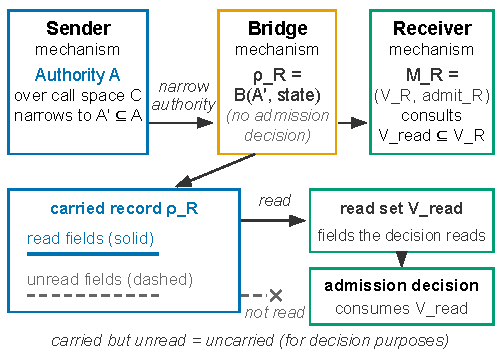
\includegraphics[width=0.95\columnwidth]{figures/figure_1_handoff_anatomy.pdf}
\caption{Anatomy of a cross-mechanism handoff. The sender narrows authority, the bridge translates it into a receiver-side record, and the receiver decides. The schematic distinguishes the record the bridge carries from the read set the receiver's decision actually consults; it carries no data and no numbers.}
\label{fig:anatomy}
\end{figure}

\subsection{The seam test and two readings}
\label{sec:readings}

The seam test is defined case-wise over the pilot-level arms. Let $\mathrm{deny}(a)$ mean arm $a$ denies the call and $\mathrm{allow}(a)$ mean it admits the call. Two predicates are reported separately:
\begin{align}
\mathrm{violation}_S(c) &:= \mathrm{deny}(1)\land\mathrm{allow}(5), \label{eq:sender}\\
\mathrm{novelty}_R(c) &:= \mathrm{deny}(2)\land\mathrm{allow}(5). \label{eq:receiver}
\end{align}
The first is sender-relative: the sender's narrowed arm denies, the composed arm admits. The second is receiver-relative: the standalone receiver denies, the composed arm admits. The seam test is the conjunction of no sender violation, no receiver violation, and a composed admission:
\begin{equation}
\mathrm{seam}(c):=\mathrm{safe}(1)\land\mathrm{safe}(2)\land\neg\mathrm{safe}(5),
\label{eq:seam}
\end{equation}
where $\mathrm{safe}(a)$ holds exactly when no call outside that arm's own world's conferred authority executes. Arm~1 carries the sender's narrowed decision, arm~2 is the receiving mechanism evaluated standalone, arm~5 is the scope-only composition, and arms~6 and~7 are the evidence and fail-closed interventions. The two predicates are reported separately because they can diverge: in Pilot~1 and the SentinelAgent pair, the sender-relative violation fires but novelty does not; in E1 under the family-wide convention both are false; under arm-native scoring both fire. Arms~6 and~7 are reported separately as repair outcomes, not folded into the predicate: a leaking repair arm is a repair failure, not a composition failure.

The distinction matters because the two questions diverge when the receiver is unsafe on its own. In Pilot~1 and the SentinelAgent pair, arm~5 admits the same calls as arm~2; the composed system commits sender-relative violations, but it adds no receiver-relative novelty. In E1 under arm-native scoring, arm~2 is safe and arm~5 admits, so both predicates fire. The result sections report both counts; a zero in the seam test is a statement about the conjunction, not about the absolute level of unauthorized admission.

\subsection{Scoring conventions and execution ledger}
\label{sec:ledger}

Every classification of an arm's admissions names the scoring convention under which it was scored. The convention set is closed and contains four members. The \emph{family-wide} convention scores every arm of a mechanism family against a shared authorization norm derived from the handoff, including arms whose own world contains no handoff. The \emph{arm-native} convention scores each arm against its own world's conferred authority. The \emph{boundary} convention scores the standalone arm canonically regardless of the surrounding variant loop variable, and scores variant arms against the authority their variant-manifest derivation produces. The \emph{SentinelAgent arm-invariant} convention applies one admission relation across all arms, including the standalone arm. Conventions are carried by disclosure rather than by report-time choice: every count names the convention that produced it.

\begin{table}[t]
\caption{Matrix execution ledger, stated as an explicit sum of enumerated components. E1's six control executions are inside the 2,446 total; the SentinelAgent and boundary control executions are outside it.}
\label{tab:ledger}
\small
\begin{tabular}{@{}>{\raggedright\arraybackslash}p{0.44\columnwidth}>{\raggedright\arraybackslash}p{0.32\columnwidth}r@{}}
\toprule
Run & Design & Executions \\
\midrule
Pilot 1 (v2), APC $\rightarrow$ TraceGrant & 80 cases $\times$ 7 arms & 560 \\
Extension E1, action narrowing + M2-auth & 8 cases $\times$ 5 arms & 40 + 6 \\
Discriminating Test 1 (re-scoring) & no new executions & 0 \\
Discriminating Test 2 & 8 cases $\times$ 2 arms & 16 \\
SentinelAgent pair, APC $\rightarrow$ SentinelAgent & 96 cases $\times$ 7 arms & 672 \\
Boundary, V1/V2 & 6 arms $\times$ 2 variants $\times$ 96 cases & 1,152 \\
\midrule
\textbf{Total} & & \textbf{2,446} \\
\bottomrule
\end{tabular}
\end{table}

Table~\ref{tab:ledger} states the ledger. The seven-arm structure used in Pilot~1 and the SentinelAgent pair is: arm~1 \code{apc_alone} (sender alone; carries the narrowed decision); arm~2 \code{tracegrant_alone} or \code{sentinelagent_alone} (receiver alone; no handoff); arm~3 \code{apc_apc_preserved} (same-mechanism preserved control); arm~4 \code{apc_apc_reset} (same-mechanism reset control); arm~5 \code{apc_*_scope_only} (composed scope-only arm; the seam-test arm); arm~6 \code{apc_*_retained} (composed evidence/attestation repair); and arm~7 \code{apc_*_fail_closed} (composed fail-closed repair). The boundary run adds arm~2v \code{sentinelagent_alone_variant}. The E1 extension uses arms~1, 2, 5, 6, and~7. Arm numbering is a role label across sets, not a claim that implementations are identical. Artifact roots are \code{v2}, \code{dt}, \code{sa}, and \code{b}; full paths remain in the artifact tree. E1's six control executions are inside the total; the SentinelAgent run's 10 control executions and the boundary run's 7 control executions are outside it, as are determinism replays and separate Pilot-1 control, replay, and latency records. No execution is counted twice.

\subsection{Threat model, ethics, and scope}

The experiments are synthetic and offline. The assets are the sender's narrowed authority, confidential markers, cumulative budget, freshness and revocation state, and audit evidence. The adversary is a caller or delegate that can present calls and tokens to the receiver within the harness, substitute recipients, widen resources, omit fields, replay calls, or mint a token with the published test key; it cannot compromise the receiver process or bypass the bridge. The trust boundary is sender $\rightarrow$ bridge $\rightarrow$ receiver. The bridge is the translation point; the receiver's own decision is trusted to run, but its read set is the object of measurement. V1/V2 are non-narrowing-preserving derivations, not a malicious bridge that forges signatures without the key. The key model is HMAC-SHA256 with a public test constant; any keyholder can mint a token the receiver verifies. Asymmetric delegation chains, direct calls that bypass the bridge, a compromised receiver, side channels, prompt injection and intent classification (H7), network attacks, and multi-hop chain reconstruction (H4) are out of scope.

AI-assisted tools were used for the experiment implementation and artifact quality assurance. These are not human peer review and do not constitute independent vendor validation. No AI system is an author; the author remains responsible for all claims, artifacts, and errors. No human-subjects data were collected; the work is synthetic and offline.

\section{Results}
\label{sec:results}

This section reports three pilots and a boundary run. Each subsection states the classification convention, the effective witness set behind every count, and the two readings defined in Section~\ref{sec:readings}. All tables are generated from the frozen result artifacts and transcribe the artifact fields verbatim.

\subsection{Pilot 1: APC to TraceGrant}
\label{sec:pilot1}

Pilot~1 is the first end-to-end pair: a sender running APC narrows its authority and hands off to a receiver running TraceGrant. The pilot separates what crosses the seam cleanly from what does not, on 80 cases across seven arms---40 attack and 40 benign cases per arm---with classifications scored under the frozen family-wide convention. The 40 attack cases are 10 templates $\times$ 4 attack parameters (8 runs each, attack and benign interleaved); the 24 leak cases of the headline arm are 6 leak templates $\times$ 4 parameters, one design point per row, not 24 independent demonstrations. Under the two readings, the pilot records 24/40 sender-relative violations (arm~1 denies, arm~5 admits) and 0/40 receiver-relative novelty (arm~2 denies, arm~5 admits), because arm~2 and arm~5 leak the same 24 cases. The zero is a statement about novelty, not about the absolute level of unauthorized admission. The pilot is a constructed case family rather than a benchmark, and no comparability with published benchmark numbers is claimed.

What is checkable is denied. The four \code{resource_widen} attacks are dropped in every arm---including both standalone mechanisms---because the sender's scope meet holds on the resource side and the narrowed set, once crossed, lets any downstream check see the widened call for what it is. The resource clause of the scope-trust claim (H1 \status{REFINED}) is therefore \status{UNTESTED}, not refuted: the case set contains no resource-side trust failure to exercise, and a zero on a caught case is not evidence that the clause is false. The two representable attack classes inside the shared vocabulary---recipient substitution and the omitted-forbidden default---are caught (leaked 0) by mapping-side canonicalization and BIND constraints rather than by effect-time detection. They are caught-case and mapping-attribution findings, not silence instances; they do not support H3. The one seeded exception is the unsatisfiable-VERIFY template, treated as a completion-integrity boundary rather than an unauthorized-effect leak and also not an H3 instance.

What leaks is the unrepresentable. Six of the ten templates leak 4 cases each under the composed M0 arm---principal rebind, composition-history loss, repeated calls (4 cases but 6 unauthorized-effect events), budget reset, expired delegation, and revoked envelope---for a total of 24 of 40 attack cases and 26 unauthorized-effect events, with confidential marker external effects recorded in 4 of those events. These are the fields of dynamic state, identity, and freshness that the receiver's decision does not consume: some are absent from its vocabulary, some are carried but unread, and some are readable but not carried (Appendix Table~\ref{tab:fieldaudit}). No decision on the receiving side reads them, so the same faithful transport that delivers resource scope correctly delivers nothing actionable about revocation or budget. Because the classes are aligned row-by-row with the six templates, the composition-type claim (H2 \status{SUPPORTED})---that dynamic state, identity, and freshness do not cross as actionable decision inputs and leak---is carried here with every count attached to its row. The cross-pair headline appears only in Section~\ref{sec:sa} and is not invoked here. Under the frozen family-wide convention, no Progent figure is used for comparison; H6 is \status{REFINED} on the two measured receiving pairs, not on an external baseline: the pair similarity is partly construction-forced (Section~\ref{sec:synthesis}).

\begin{table}[t]
\caption{Pilot-1 arm outcomes: attack cases leaked, unauthorized-effect events, and benign false-denial cases per arm. The same-mechanism reset control \code{apc_apc_reset} records 8 leak cases and 8 events on the shared 80 cases.}
\label{tab:pilot1}
\small
\begin{tabular}{@{}lrrr@{}}
\toprule
Arm & Attack leaks & Events & Benign FD \\
\midrule
\code{apc_alone} & 0 & 0 & 0 \\
\code{tracegrant_alone} & 24 & 26 & 0 \\
\code{apc_apc_preserved} & 0 & 0 & 0 \\
\code{apc_apc_reset} & 8 & 8 & 0 \\
\code{apc_tracegrant_scope_only} & 24 & 26 & 0 \\
\code{apc_tracegrant_retained} & 0 & 0 & 0 \\
\code{apc_tracegrant_fail_closed} & 0 & 0 & 20 \\
\bottomrule
\end{tabular}
\end{table}

Table~\ref{tab:pilot1} summarizes the per-arm outcomes. The standalone receiver recorded 4 receipt failures (\code{v2/raw_metrics.json}, \code{tracegrant_alone.receipt_failures = 4}); this control detail is not part of the 24/40 leak count and is not load-bearing for H2. M0 is this program's one-step, transport-faithful bridge---a design choice of this implementation, not a defect of APC or TraceGrant as published. The composed arm with M0 (\code{apc_tracegrant_scope_only}) exhibits leak counts and event counts identical row-by-row to the standalone receiver: the handoff does not add a dynamic-state leak class, it fails to remove the receiver's own. That identity is construction-forced and carries no evidential weight about composition (Section~\ref{sec:synthesis}); the informative rows are the remaining arm comparisons. The arm that carries the sender's decision as an evidence record with a consistency digest (\code{apc_tracegrant_retained}, M2) shows 0 leaked attack cases and no false denials. M2 did not sign the record: it was trusted harness input with a consistency digest. HMAC-signed M2-auth is introduced only in E1, and signature verification under a trusted key belongs to E1 M2-auth and to the SentinelAgent pair's arm~6. The 0/40 result therefore measures carriage of the upstream decision, not signature verification. The arm that refuses to translate what it cannot represent (\code{apc_tracegrant_fail_closed}) also shows 0 leaked cases, at a measured utility cost: 20 of 40 benign cases are falsely denied, in 28 distinct events.

The state/identity rows are the pilot's H3 observation, narrowed to a field-level account: silent non-enforcement, not crashes or misparses. The receiver admits these calls with no parse error, no gate code, and no effect-time detection, because the fact that should have denied has no column in the receiver's decision. The broader claim that vocabulary gaps generally manifest as silence is not tested; the audited fields are in Appendix Table~\ref{tab:fieldaudit}. The resource and caught-action rows are not H3 evidence.

\subsection{Extension E1 and the resolving tests}
\label{sec:e1}

Pilot~1 severe cases all sit on the state/identity side, so E1 asks the same question of a fact the receiver's vocabulary demonstrably does represent: the action. E1 isolates one design point---a \code{send_external} call inside the sender's root set but outside the narrowed action set that crossed the seam---replicated across four attack cases on an axis the construction neutralizes (recipient value, budget); the four benign cases are context, and the effective sample size is 1 design point $\times$ 4 attack cases. The experiment spans 8 cases $\times$ 5 arms = 40 executions plus 6 control executions on a separate denominator (the 6 are counted in the 2,446 ledger but excluded from the 40-case E1 denominator), scored under the frozen family-wide reference convention. Under the two readings, E1 records 4/4 sender-relative violations; receiver-relative novelty is 0/4 under the frozen family-wide convention and 4/4 under the arm-native convention. The reference oracle for this family is family-wide: it scores arm~2, which contains no handoff, against the handoff-derived norm---an authority-assignment convention for the standalone arm that is disclosed rather than hidden, and one that the first resolving test re-scores.

The result decomposes transport from admission at the action field. The narrowed action set crosses the seam intact---the synthesized record in the composed arm carries exactly \code{[read_public, save_internal]}---and the composed arm still admits the four attacks, 4/4, with 4 unauthorized-effect events; the record's action field is present in the snapshot and unread by the synthesis. This is the action-clause instance of the scope-trust claim (H1 \status{REFINED}), measured here: an authorization-carrying fact crosses the seam and a secondary receiving decision never reads it. In the frozen family-wide scoring the same 4/4 leaks appear in arm~2, which contains no handoff; the two M0 arms are scored identically and leak identically. The sender-relative reading is 4/4 in both conventions; the receiver-relative reading is 0/4 under the family-wide norm and 4/4 under the arm-native norm, because arm~2's own-world authority differs from the handoff-derived norm. The four attack cases are \code{action_narrow-0-a} through \code{action_narrow-3-a}, and the four benign cases are \code{action_narrow-0-b} through \code{action_narrow-3-b}.

\begin{table}[t]
\caption{E1 per-arm outcomes on the 4 attack and 4 benign cases. Arm~6 denies 4/4 attacks with \code{PROOF-GAP}, and all 8 signed records (4 attack, 4 benign) verify \code{EVIDENCE-VERIFIED}; that cell is report-only in the frozen metrics output (Section~4.2).}
\label{tab:e1}
\small
\begin{tabular}{@{}>{\raggedright\arraybackslash}p{0.47\columnwidth}rrr@{}}
\toprule
Arm & Attack leaks & Events & Benign FD \\
\midrule
1 \code{apc_alone} & 0/4 & 0 & 0/4 \\
2 \code{tracegrant_alone} & 4/4 & 4 & 0/4 \\
5 \code{apc_tracegrant_scope_only} & 4/4 & 4 & 0/4 \\
6 \code{apc_tracegrant_retained} & 0/4 & 0 & 0/4 \\
7 \code{apc_tracegrant_fail_closed} & 0/4 & 0 & 0/4 \\
\bottomrule
\end{tabular}
\end{table}

Three mechanism-level facts sit alongside Table~\ref{tab:e1}. First, the arm-5 confusion matrix on the eight-case family is TP~4, FP~0, FN~0, TN~4---precision 1.0, recall 1.0 under this experiment's own contract. The matrix is construction-consistent rather than an independent estimate: the four attack cases are built to be outside the narrowed action set, and the four benign cases are built to be inside it, so the scores record that the harness applied its own labels consistently. The substantive result is the admission pattern, not the precision/recall figure. This is a representable-but-unread consumption failure, reported under H1 \status{REFINED} and the formal core, not H3. Second, the evidence arm (\code{apc_tracegrant_retained}) denies all four attacks (\code{PROOF-GAP} after the shadow APC denies) while verifying the signed record on all four attack cases; the eight signed records across arm-6 runs---four attack and four benign---are all \code{EVIDENCE-VERIFIED}. This cell is report-only in the frozen metrics output: the raw field traces for signed-record admission codes are not stored in \code{v2/extension_e1/metrics.json}, and the count is carried from the frozen report's evidence-auth column (\code{v2/EXTENSION_E1_RESULTS.md} Section~3.4). Third, the three controls---\code{C-valid}, \code{C-mutated}, \code{C-replay}---each with a failure probe, pass 3/3 across 6 executions on their own denominator, all \code{lock_matches} true; they are not mixed into the 40-case run. The signing scheme is HMAC-SHA256 over a canonical payload with a 56-byte key and is disclosed as a public test constant; M2-auth assumes attestation is verified under the trusted key and does not establish authenticated transport. The dataset hash of the locked 8-case set is \code{1b7c6083...b2e264ba} (design locks, not reseals).

Two pre-registered resolving tests settle where the action-clause violation is located and how it is repaired. Test~1 is scoring-only---zero new executions---and re-scores the four frozen arm-2 attack records against two authority conventions: the frozen family-wide handoff norm, under which arm~2 leaks 4/4, and the arm-native root norm, under which arm~2 leaks 0/4. On the same frozen records, the sender-relative count (arm~1 denies, arm~5 admits) is 4/4 under both conventions; the receiver-relative count is 0/4 under the family-wide norm and 4/4 under the arm-native norm. The classification is therefore measured to be convention-dependent, and the convention-dependence is itself the finding: the composition-specific reading rests on the arm-native scoring of arm~2, which both resolving tests adopt going forward. Under that reading the action-family exception to the pair-similarity finding (H6 \status{REFINED}) is composition-specific: on this family, this arm, this mechanism---arm~1 denies, arm~2 is safe, arm~5 leaks, with no claim about other families. The seam test as operationalized here is a widening test; it can fire only where the composition widens, and a zero where the composition does not widen does not by itself establish composition-independence.

Test~2 measures the repair (M0-A consumption rule): making the synthesized read set consume \code{snapshot.actions} denies all 4 attacks on action scope in the composed arm while allowing all 4 benign cases, with 12/12 admitted-call receipts verifying and 0 false denials, all under 16 sequential executions. The arm-2 control in the same loop is unchanged: gate outcome parity 8/8 with canonical, and the synthesized contract digests byte-identical on all 8 cases, so the variant changes admission handling only, not the M0 arm's own decisions. All 10 pre-registered predictions across the two tests match; the lock hash is \code{8cd4d993...996011ab}. This is the measured consumption-side instance of the formal core's repair rule (Section~\ref{sec:formal}): the receiver must consume the narrowed action set it is handed. The Test~2 runner-hash disclosure is recorded: \code{dt/test2_manifest.json} records \code{runner_sha256_matches_mini_lock: false}; the earliest full run crashed while assembling the reconciliation after writing the test artifacts, and the corrected runner re-ran the complete matrix. The mini-lock, cases, arms, and predictions were unchanged; the manifest's \code{bookkeeping_note} records the deviation, and no measurement or reported count changes.

Read together, Pilot~1 and the E1 resolving tests measure two loci. At the state/identity locus, the vocabulary gap is absolute and the leak count is the standalone count; sender-relative violations are 24/40 and receiver-relative novelty is 0/40. At the action locus, the sender-relative count is 4/4 under both conventions; the receiver-relative count is 0/4 under the frozen family-wide convention and 4/4 under the arm-native convention, and consumption---the receiver reading the fact it was already handed---closes the violation without disturbing the rest of the synthesis.

\subsection{SentinelAgent pair: APC to SentinelAgent}
\label{sec:sa}

The second receiving pair re-runs the composition program against SentinelAgent's delegation-token vocabulary: the locked bridge mints one delegation token per attempted call, and the receiving side executes the pinned prototype's own token checks. Every classification here names its convention, which is the pair's arm-invariant scoring: scopes are intersected with the receiving manifest and the composition term is applied to arm~2 as well, although arm~2's world contains no handoff. Under a rescoping of the composition term to the handoff arms alone, the arm-2 \code{composition_history_loss} cells would read safe rather than leak, so the pair's arm-2 and arm-5 readings are one convention's readings. The witness structure is 12 templates $\times$ 8 runs, executed as 96 cases $\times$ 7 arms = 672 strictly sequential, offline, deterministic runs over 48 attack cases. Under the locked convention the pair records 28/48 sender-relative violations and 0/48 receiver-relative novelty, because arm~2 and arm~5 leak the same 28 cases. The self-review re-verified the lock and case-set hashes unchanged after the run and re-measured determinism with 20 re-executions and zero mismatches.

Under the locked convention the standalone receiving arm and the composed scope-only arm leak the same 28 of the 48 attack cases and emit the same 30 unauthorized-effect events. Their leak sets are identical by construction---same contract, same scoring, composition changing only which vocabulary handles the prelude calls---and we carry the identity as forced, not as evidence. The dynamic-state classes of the first pair repeat and dominate: 24 of the 28 leaks are principal/task identity (4 cases), composition history (4), repeated calls (4 cases with 6 events), cumulative budget (4), expiry (4), and revocation (4). This is the structural account for H3 \status{REFINED}: the audited state/identity aspects fail silently, but through three distinct loci---carried-but-unread (expiry), read-but-not-carried (revocation), and absent from the admission read set (principal/task, composition history, budget, replay). The original broad wording, that vocabulary gaps generally manifest as silence, is not tested; the field audit is Appendix Table~\ref{tab:fieldaudit}. The remaining 4 signature-family leaks are not H3 evidence; they are treated under H5/H6 below. The receiver-relative seam test again returns zero under the locked conventions---no case is safe in both mechanism-alone arms and admitted under composition in this pair.

The run's own integrity record is not uniformly green: the SentinelAgent manifest records \code{expected_vs_observed_ok = false}, and its metrics record \code{comparison.overall_ok = false}. The two failed checks are the false-denial-event lock (26 locked, 28 observed) and the arm-5 confusion true-negative denominator (68 locked, 20 observed on the attack-case basis); both are recorded verbatim in \code{sa/sa/reconciliation.json} with \code{affects_behavior_cells: false}. The first is a derivation undercount: the lock enumerated only first calls of two \code{repeated_calls} cases, while each case produces two false-denial events under the locked definition, which yields 28. The second is a denominator slip: the lock used the all-96-case denominator for TN (48 benign + 20 caught attacks), while the metrics code computes TP/FP/FN/TN over the 48 attack cases (TN = 16 rejected + 4 allowed-no-effect); TP/FP/FN are 28/0/0 either way, and $28+20=48$, $28+68=96$. Neither changes a behavior cell or a reported leak count.

The two remediations carry measurable prices, and the pair headline is the frozen H2 claim: the repair is carrying the upstream decision, not a check inside the receiver's vocabulary (H2 \status{SUPPORTED}). In this pair the evidence arm records zero attack successes and zero false denials against the scope-only arm's 28 leaks. The fail-closed arm also records zero leaks, by refusing dynamic state it cannot translate, at a measured utility cost: 20 benign cases rejected and 28 false-denial events. The trust conditions are part of the finding: the evidence arm reads the signed attestation as verified under the trusted key, and the fail-closed arm accepts its 20 benign refusals deliberately---both scoped design choices of the mapping, neither claimed production-safe. H6 \status{REFINED} reads the same evidence pair-wise: within the measured pairs, the state/identity leak shapes are similar, but the similarity is partly an artifact of shared case templates and shared scoring; it is not a general cross-pair law. The differences that exist are remediation mechanics---signed attestation here, digest-only evidence carriage and receipts in the first pair---plus the one new standalone class the token ecosystem contributes.

The signature family is this pair's measurement of H5 and its first end-to-end test. Its witness structure is 2 pairs $\times$ 4 document parameters $\times$ 2 variants = 16 cases (8 attack, 8 benign), each executed across the 4 token arms. A token whose content would pass the checks but which is signed with the prototype's published key constant instead of the trusted harness key is rejected \code{SIGNATURE_INVALID}---4 rejections per token arm, and not counted as a false denial under the locked scoring rule. Verification without the key cannot admit; verification with the key attests something narrower than authority. Delegate-minted tokens are admitted exactly like bridge tokens wherever the prior authorization is not restored, and a control presenting identical tokens attributed to two distinct minters returns identical codes. Within the token vocabulary, any keyholder is to the receiver equivalent to the issuer, and the frozen wording of H5 \status{REFINED} states the measured boundary for this pair: a validly-signed token attests to integrity and key possession, not source of authority---scoped to this pair, with the trust-boundary caveat that the pair exercises one prototype, one key model, one case family, and the ``or a call to the DAS'' alternative was not exercised end-to-end. The same property generates the pair's one new leak class: \code{keyholder_widen}, in which a caller-held delegate writes a manifest containing the widened resource and the token arms admit it 4/4---a token-ecosystem standalone class (H6 \status{REFINED}) rather than a composition failure, and the observation that makes key distribution the critical interface of this seam.

Ten controls pass across the family---signature-validity failure probes, foreign-key rejection, two-minter indistinguishability, attestation tamper and replay---showing the checks are neither vacuous in the admit direction nor no-ops in the deny direction. Across the 7-arm, 96-case matrix, 756 evaluated events decompose exactly as $756 = 488$ admissions $+ 150$ token-attached denials $+ 118$ denials without a token key. The 150 token-attached denials are 40 native P6/P7 denials, 42 attestation-stage denials in arm~6, and 68 pre-presentation refusals in arm~7. Of the 488 admissions, 230 carry no token key. The non-vacuity count is $638 = 488 + 150$; the 118 denials without a token key are outside it.

\subsection{Boundary: non-narrowing-preserving bridge variants}
\label{sec:boundary}

The boundary run asks the reversed question: not whether a faithful bridge drops facts, but what happens when the bridge's own manifest derivation is not narrowing-preserving. V1 derives the receiving manifest from the delegate's pre-narrowing role scope rather than the post-handoff effective scope; V2 fills an omitted-recipient default into the manifest's SEND endpoint (\code{forbidden-default@example.test}). Neither derivation consumes a fact the sender conferred; both widen. Each classification names its convention: arm~2 remains canonical regardless of the variant loop variable, and the variant arms consume the variant manifest derivation. The boundary records 4 new sender-relative cases per variant; receiver-relative novelty is 4/4 against the canonical receiver and 0/4 against the variant receiver, so the new cases are bridge-attributable. The run executes 6 arms $\times$ 2 variants $\times$ 96 cases = 1,152 strictly sequential runs, 96 rows per arm-variant cell; 7 controls pass, and the self-review records \code{ok} with the harness and case-set hashes unchanged, while the boundary lock hash is recorded in \code{manifest.json.lock}. Its attack structure is deliberately thin: 1 design point $\times$ 4 cases per variant---the four \code{resource_widen} attacks under V1, the four \code{omitted_forbidden_default} attacks under V2---so its 8 attack cases in total are not 8 independent designs.

Both derivations produce the predicted widening, with and without composition. Under V1 the composed arm leaks the 4 \code{resource_widen} attacks, among them the widened resource \code{docs:external/secret}, which the canonical arm~2 blocks; under V2 the composed arm leaks the 4 \code{omitted_forbidden_default} attacks. The counts follow the delta convention: arms 2v and 5 leak 32 cases and 34 unauthorized-effect events per variant, arm~2 leaks the canonical 28 cases and 30 events, and the difference is the 4 new cases; $32=28+4$. The 32/32 identity between arm~2v and arm~5 is an identity of leak sets, not a claim that all 96 cases leak. Arm~1 leaks none in either variant. The receiver-relative seam counts follow the same shape: 4 per variant against canonical arm~2. Because the standalone variant arm~2v leaks the identical set per variant---forced by construction, not evidence---the seam test fires, but its firing carries no composition-specific witness. The informative contrasts are canonical arm~2, safe on the variant cases, against composed arm~5, leaking them; and arm~2v, leaking, against arm~2, safe.

The attribution is measured, in the frozen wording: the failure is the bridge's manifest derivation, not composition. The receiver cannot recover a fact the derivation did not narrow---the frozen derivation-side clause. H1 \status{REFINED}: the bridge's manifest derivation extends scope trust---the receiver reads the signed manifest as authority---and the refinement lands on the derivation layer. H2 \status{SUPPORTED} is unchanged: V1 and V2 add no new dynamic-state class, and their new leaks are scope/manifest-derivation classes. These are derivation-widening findings under H1 \status{REFINED} and H6 \status{REFINED}, not H3: both mismatches are faithful to what the bridge wrote into the manifest---a role scope exceeding the root grant under V1, a default-filled send endpoint under V2. H5 \status{REFINED} now covers the keyholder property at the bridge/manifest layer: a bridge holding the key can write a widened manifest or a default-filled endpoint, and the receiver admits what it verifies. H6 \status{REFINED}: a bridge-design artifact, not a composition-specific failure.

Arms~6 and~7 suppress the widened calls rather than repair them. The evidence arm denies the 4 variant cases as \code{APC-DENY} per variant, with zero leaks; the fail-closed arm denies them as \code{SHADOW-DENY} $\times4$ per variant, with zero leaks and its measured cost of 20 benign false denials and 28 false-denial events. No benign case is falsely denied in arms~1, 2, 2v, 5, or~6, and the no-divergence control (CV1b) confirms the variant manifests match canonical on the benign cases that should not diverge. The missing step is not receiver consumption here; the derivation is at fault.

The receiver-relative zero survives, bounded. It is a property of narrowing-preserving mappings (canonical T0) on the frozen case sets and does not extend to non-narrowing-preserving derivations (Section~\ref{sec:formal}). The run's manifest check is narrow, recorded verbatim: \code{expected_vs_observed_ok = true} checks the seam count only. One locked statement was overbroad and is reconciled rather than edited: arm~2 was stated as safe on all cases, and it is safe on the variant-specific cases per variant while carrying the pre-existing canonical leak set elsewhere. V1 and V2 are two derivations tested in one pair's token vocabulary; they are not asserted to be typical, nor the only or most likely bridges.

\subsection{Cross-cutting synthesis}
\label{sec:synthesis}

The cross-cutting claim is a refinement, not a universal zero. Two readings are reported for every set: sender-relative violation (arm~1 denies, arm~5 admits) and receiver-relative novelty (arm~2 denies, arm~5 admits). Table~\ref{tab:readings} collects the counts; Appendix Table~\ref{tab:fieldaudit} audits the state/identity fields; the claim statuses are collected in the text below.

\begin{table*}[t]
\caption{Two readings of the seam test: sender-relative violation and receiver-relative novelty by experiment set. Counts are attack-case counts, not execution counts; the 2,446-execution ledger is Table~\ref{tab:ledger}. ``0/40'' and ``0/48'' are novelty zeros, not zeros of sender-relative violation.}
\label{tab:readings}
\small
\begin{tabular}{@{}>{\raggedright\arraybackslash}p{0.16\textwidth}r>{\raggedright\arraybackslash}p{0.15\textwidth}>{\raggedright\arraybackslash}p{0.15\textwidth}>{\raggedright\arraybackslash}p{0.35\textwidth}@{}}
\toprule
Experiment set & Attack cases & Sender-relative violation & Receiver-relative novelty & Construction note \\
\midrule
Pilot 1 (APC $\rightarrow$ TraceGrant) & 40 & 24/40 & 0/40 & Arm~2 and arm~5 leak the same 24 cases; the identity (24/24 cases, 26/26 events) is forced by shared contract and scoring \\
SentinelAgent pair & 48 & 28/48 & 0/48 & Arm~2 and arm~5 leak the same 28 cases; the identity (28/28) is forced \\
E1, family-wide scoring & 4 & 4/4 & 0/4 & Arm~2 leaks 4/4 under the handoff norm \\
E1, arm-native scoring & 4 & 4/4 & 4/4 & Arm~2 is safe (0/4); the only genuine composition-specific test \\
Boundary V1, canonical arm~2 & 4 variant attacks & 4 new / 4 (32/96 total) & 4 new / 4 & Arm~2v leaks the same 4 new cases; receiver-relative novelty against arm~2v is 0, so the 4 new cases are bridge-attributable \\
Boundary V2, canonical arm~2 & 4 variant attacks & 4 new / 4 (32/96 total) & 4 new / 4 & Same shape as V1 \\
\bottomrule
\end{tabular}
\end{table*}

The first two rows carry the program's main negative result: the composed arms commit sender-relative violations on 24/40 and 28/48 attacks, but they add no receiver-relative novelty, because the standalone receivers leak the same calls. The zero is a statement about composition, not about safety: the sender's narrowing is not enforced, and the receiver is already unsafe on its own. The two pair-pilot zeroes are construction-forced identities of arm~2 and arm~5; they carry no evidential weight about composition. The E1 family-wide zero is a third pair-level zero, but it is convention-dependent rather than construction-forced: the same records give 4/4 under arm-native scoring. The boundary's composition-specific zero is a separate identity between arm~2v and arm~5, and the four new cases per variant are bridge-attributable. E1 is the only genuine composition-specific test in the program: arm~2 is safe under arm-native scoring, arm~5 admits 4/4, and the consumption repair reverses the admission pattern. Its result is one design point $\times$ four attack cases and is convention-dependent.

The formal core (Section~\ref{sec:formal}) supplies the vocabulary for these observations: the blindness observation is definitional, and the seam proposition's clauses are measured rather than proved. The observation says that if the receiver's admission depends on the call only through its read-set projection, and no value in that read set separates the narrowed set from its complement on a call pair, then no admission function over the read set can enforce the narrowing on that pair; its corollary is the program's aphorism, carried but unread = uncarried for decision purposes. The measured instances recur with effective $n$ attached: in E1, the narrowed action set crossed the seam intact and the synthesis did not read it, and the consumption repair reversed the counts (Table~\ref{tab:e1}); in the SentinelAgent pair, the state/identity aspects fail through the three loci in Appendix Table~\ref{tab:fieldaudit}, with the witness set 6 leak templates $\times$ 4 parameters = 24 attack cases of 48; in the boundary run, the widened manifest is admitted by the receiver standalone and composed---the bridge wrote the widened scope, so there is no consumption failure to repair at the receiver, and the derivation is the fault.

Those instances motivate the two repair loci. Receiver side, when the fact crossed intact: carry the upstream decision as evidence---signed attestation in the SentinelAgent pair, where the evidence arm eliminates all 28 leaks while recording no false denials itself; HMAC-signed M2-auth in E1, where the scheme denies 4/4 attacks; digest-only evidence carriage in Pilot~1---or retain the upstream denial, as the fail-closed arms do at their measured benign costs---with consumption, not carriage, as the part that enforces. Derivation side, when the bridge itself widened: fix the manifest derivation at the bridge, so that the derivation preserves the narrowing. Figure~\ref{fig:repair} places the two loci in one picture.

\begin{figure}[t]
\centering
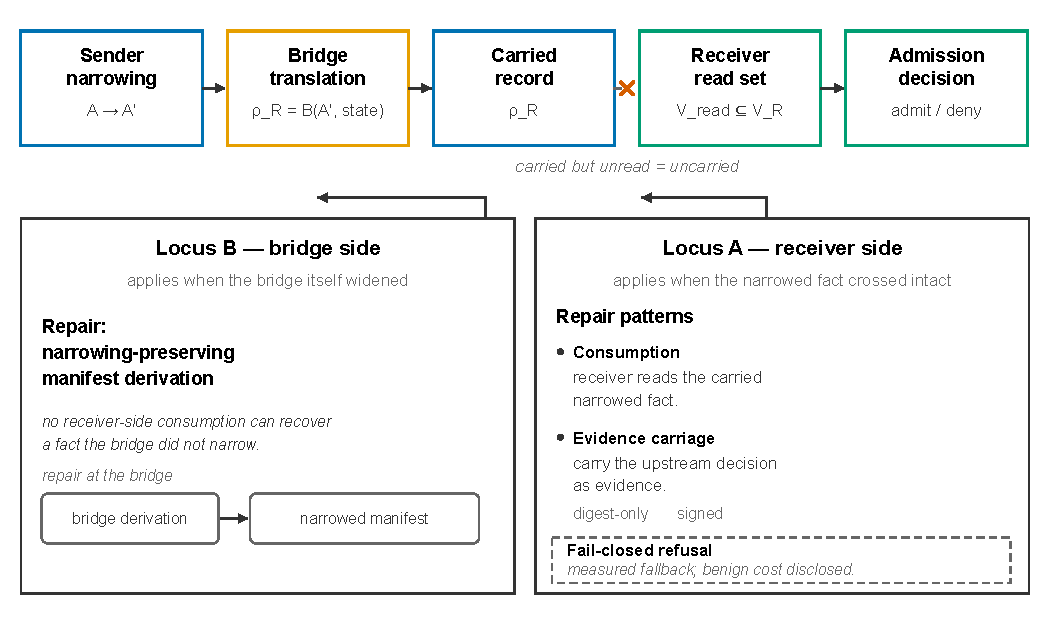
\includegraphics[width=0.9\columnwidth]{figures/figure_2_repair_loci.pdf}
\caption{Where the decision can be rescued: the two repair loci of the seam program (schematic; no data). Locus~A sits at the receiver's admission step and applies when the narrowed fact crossed intact; Locus~B sits at the bridge's derivation step and applies when the bridge itself widened. The annotation ``carried but unread = uncarried'' labels the gap between the carried record and the receiver's read set.}
\label{fig:repair}
\end{figure}

No unconditional reading is available from these runs, and each sentence above is bounded the way its evidence is: by its scoring convention, by its case set, and by the trust model of the arm it describes. The two-count reading is the paper's main methodological correction: a zero in receiver-relative novelty is not a zero in sender-relative violation, and the difference is where the repair question lives.

\section{Discussion}
\label{sec:discussion}

\textbf{The practical question.} When does a composed arm admit a call the sender's narrowing denies, and when does composition add an admission beyond what the standalone receiver already exhibits? The anatomy is familiar: a sender narrows authority, a bridge translates the narrowed decision plus state into a receiver-side record, and the receiver decides from that record. No party owns the seam. The measured answer is bounded: the composition-specific case is one family (the E1 action family), one scoring convention (arm-native), and the frozen case sets; the sender-relative violations are broader (24/40 and 28/48) but are not composition-specific. It is not a general claim about seams, and no production-safety claim is made for any repair arm.

\textbf{Where the composed arm alone admits.} On the E1 action family, under arm-native scoring, the violation exists only in the composed arm. Arm~5 (M0 from the post-handoff snapshot) leaks \code{send_external} on 4/4 attacks, 4 unauthorized-effect events in total. Arm~1 (APC after the narrowed handoff) denies 4/4 with APC reason \code{action send_external not in scope}. Arm~6 (M2-auth signed evidence) denies 4/4 with \code{PROOF-GAP}, and all 8 signed records verify \code{EVIDENCE-VERIFIED}. Arm~7 (shadow denial retained) denies 4/4. Benign calls are allowed 4/4 in every arm, zero false denials. The attributable locus is the receiver's synthesis: arm~5's snapshot carries the narrowed action set \code{actions = [read_public, save_internal]} yet M0 never consumes the action field---carried but unread is uncarried for decision purposes (Section~\ref{sec:formal}). Under the frozen family-wide convention the arm-2 and arm-5 leaked sets are identical; under arm-native scoring arm~2 is safe and that identity no longer holds. The family-wide identity is forced by construction and carries no evidential weight about composition; it is disclosed as a convention, not evidence.

\textbf{Repairs.} Four loci follow: three receiver-side (evidence carriage, retain the upstream denial, consumption) plus the derivation-side rule from Section~\ref{sec:formal}. \emph{Evidence carriage}: in the SentinelAgent pair, arm~6 (signed attestation) closes all 28 baseline leaks with 0 leaks and 0 false denials; in E1, arm~6 (M2-auth) denies 4/4 attacks; in Pilot~1, arm~6 carries the decision as a digest-only record and closes the 24/40 baseline leaks. The caveat is load-bearing: the signed arms assume the attestation is verified under the trusted key, and M2-auth narrows tamper and replay but does not establish authenticated transport---the signer is the same harness that was the original trust anchor, and any holder of the public test key can mint valid records. Evidence carriage is therefore a fix only relative to a correctly deciding upstream. \emph{Retain the upstream denial}: Pilot~1 arm~7 records 0 leaks on 40 attack cases, 20/40 benign false-denial cases, 28 false-denial events; SentinelAgent arm~7 records 0 leaks, 20 benign false-denial cases, 28 false-denial events; boundary arm~7 records 0 leaks, \code{SHADOW-DENY} on the 4 seam cases per variant, 20 benign FD cases and 28 FD events. The utility cost is real and measured. \emph{Consumption}: E1 Test~2 denies 4/4 attacks on \code{ACTION-SCOPE}, allows 4/4 benign, records 0 false denials, and leaves the arm-2 control byte-identical---the narrowing-preserving meet's receiver-side half. Make the sender's boundary readable at the receiver and then read it: deny when the action snapshot is absent or empty, deny when the requested tool is outside the carried action set, otherwise run the unchanged synthesis. Evidence carriage is the transport; consumption is the enforcement. \emph{Derivation-side narrowing-preserving meet}: when the bridge itself widened the manifest (V1/V2), no receiver-side rule can recover a fact never narrowed. Boundary arm~5 leaks 32 cases and 34 events, which decompose as 28 pre-existing canonical leaks plus the 4 new cases per variant ($32=28+4$); standalone arm~2v leaks the identical 4 per variant; canonical arm~2 is safe on the variant-specific cases; arms~6/7 suppress with \code{APC-DENY}/\code{SHADOW-DENY} $\times4$ per variant; seam count is 4 per variant. Composition neither creates nor removes the failure: the identical admissions appear standalone in the variant arm. The fault is the bridge's manifest derivation---V1 widens role scope beyond root $R$, V2 default-fills the SEND endpoint---so the repair belongs at the bridge, not the receiver.

\textbf{Keyholder finding (H5).} Signature verification attests key possession and payload integrity, not who minted the record; any keyholder is equivalent to the issuer within the token vocabulary. This holds for delegate-minted tokens---\code{keyholder_widen} admitted 4/4 in arms~2/5---and for the bridge's own manifest derivation (V1/V2). SA signature controls: 4 \code{SIGNATURE_INVALID} per token arm for foreign-key probes; all 10 controls passed. Key distribution is the seam's critical interface: integrity plus key possession is not source of authority, so trusting a signature is not the same as trusting the minter.

\textbf{Positioning and statuses.} This paper offers a replication package and a repair taxonomy. The package contains the frozen case sets, harnesses, locks, and the locked-prediction protocol so that an independent reader can re-run the measurements; it is a release candidate, not a conformance service, certification, or benchmark, and it reports what a mapping carries rather than fixing it. The design rule is narrowing preservation at the mapping layer, with the measured receiver-locus repair (consumption) applied when the fact crossed intact and the bridge-level fix (derivation) applied when it did not. Statuses: H1 \status{REFINED}; H2 \status{SUPPORTED}; H3 \status{REFINED}; H5 \status{REFINED}; H6 \status{REFINED}; \seamstar{} \status{REFINED}; H4 and H7 \status{UNTESTED}. Receiver-relative novelty zero holds only for narrowing-preserving mappings (canonical T0) on the frozen case sets. Sender-relative violations are 24/40 and 28/48 and are not zero. The two pair-pilot zeroes are construction-forced; E1 is the only genuine composition-specific test, and it is convention-dependent (family-wide 0/4 vs.\ arm-native 4/4), one family, 1 design point $\times 4$. H1's resource clause is \status{UNTESTED}; H3 is field-level; H6 pair similarity is partly construction-forced. Arm~6 assumes attestation verified under the trusted key; arm~7 accepts 20 benign false denials; neither arm is production-safe; M2-auth does not establish authenticated transport. No claims beyond the frozen sets.

\section{Related Work}
\label{sec:related}

\textbf{Upstream formal spines.} APC's Composition Soundness (Theorem~4.7) is intra-session composition of action sequences, conditional on a complete effective restriction set, serialized admission, and static $X$---a within-mechanism guarantee, not a cross-mechanism composition guarantee. TraceGrant's soundness is assumed (Eq.~10), not proven. SentinelAgent's Theorem~4 is composition safety for two chains that both satisfy P1--P7 within its own framework; it does not cover a chain handed to a different mechanism's decision procedure. None of the three covers cross-mechanism composition as this program defines it: sender narrows, bridge translates, receiver decides, with no owner at the seam. Each guarantee stops at its own boundary. This paper's narrowing-preservation rule plus the blindness observation addresses the question the three guarantees leave open: the moment authority crosses from one mechanism's vocabulary into another's. No upstream mechanism is claimed broken or failing; all upstream figures remain their authors' self-reports, and ``reports'' is the operative word, never ``achieves.''

\textbf{Positioning anchors.} The established authorization literature supplies much of the vocabulary this measurement uses, and the paper does not claim to extend it. OAuth 2.0 token exchange standardizes delegation across security domains, and rich authorization requests carry structured, fine-grained permission requests \cite{rfc8693,rfc9396}; the seam studied here is a translation between such a request and a receiver's local decision. Macaroons make attenuation explicit through contextual caveats that a holder can append without contacting the issuer \cite{macaroons}; the present work asks whether the receiver's admission reads the caveats or narrowed facts that a bridge carries. Object-capability systems treat authority as unforgeable references and analyze composition and confinement \cite{miller,blaze}; proof-carrying authentication and SPKI certificate theory explore evidence and certificate chains that a verifier can check \cite{appel,rfc2693}. Relationship-based access control derives decisions from relationships and policy, including policy composition \cite{fong}. These lines answer how to express, attenuate, discharge, or verify authority; this paper asks an empirical question about whether a cross-mechanism handoff consumes the facts that carry the narrowing. The anchors are not baselines, no numbers are compared, and no novelty claim is made over them.

\textbf{Progent and MasDrift.} Progent is a close related work on monotonic confinement inside a single privilege-control layer \cite{progent}. No Progent figure is reproduced, re-measured, or compared; no Progent result is treated as an input or baseline. MasDrift studies authorization preservation across multi-agent coordination architectures using benign productivity tasks \cite{masdrift}. Our narrower question concerns executions through two specific public authorization artifacts and their argument-binding paths; the small deterministic matrix is a conformance study, not an architecture benchmark and not a substitute for MasDrift's broader evaluation. No MasDrift number is reproduced, re-measured, or compared.

\textbf{Industry and standards pointers.} Noma (April 2026) is cited as an adjacent industry framing of inter-agent trust at handoffs; the IETF draft (revised August 2026) is cited as a related cross-domain authorization-sharing proposal; arXiv:2605.05440 is cited as a related reference in the same area \cite{noma,ietf,tallam}. These are pointers only: their bibliographic identities were checked, but their claims are unverified and none is treated as a verified fact, a benchmark, a reproduced result, or a verified input to this manuscript. The frozen claim set governs if any pointer differs from it.

\textbf{Scope of positioning.} The section positions the paper against the three measured formal spines, two related works (Progent and MasDrift), and the established authorization literature named above. It does not survey the broader delegation and capability literature beyond those anchors, makes no novelty claim over that literature, and treats none of those systems as a baseline. A comparative treatment would require additional verified references and is not undertaken here. The reference list is correspondingly short; it is a scope limitation, not a claim that the cited set is comprehensive.

\section{Threats to Validity}
\label{sec:threats}

\textbf{Construct threats.} The case sets are constructed witnesses, not benchmarks. The first pilot family is 10 templates $\times$ 8 runs and the SentinelAgent family is 12 templates $\times$ 8 runs, each written for this program and frozen before any run. Their structure, not their scale, is what licenses a reading: E1 rests on a single design point with a neutralized parameter axis, measured as 1 design point $\times$ 4 attack cases, and the boundary run rests on two design points, each $1\times4$ cases---8 attack cases in total, which are not 8 independent cases. Convention dependence is a construct threat as much as a disclosure. The E1 receiver-relative count is 0/4 under the frozen family-wide convention and 4/4 under the arm-native convention; the sender-relative count is 4/4 under both. The convention was locked and disclosed, not chosen after the fact. SentinelAgent scoring is arm-invariant, and rescoping it would flip \code{composition_history_loss} arm~2 from leak to safe. At the boundary, arm~2 is always canonical regardless of the variant loop variable while the variant arms use the variant manifest derivation, so the identity of arm~2v with arm~5 per variant is forced by construction. The composed arm's absolute count is accordingly $32=28+4$---the pre-existing canonical set plus the per-variant new cases. Three forced identities---Pilot~1 arm~2 $\equiv$ arm~5 at 24/24 leaked cases and 26/26 events, SentinelAgent arm~2 $\equiv$ arm~5 at 28/28 leaked cases, and boundary arm~2v $\equiv$ arm~5 at 32/32 leaked cases per variant---are identities of leak sets, not claims that every case leaks; they carry no evidential weight about composition and are labeled forced.

Two operational caveats complete the construct picture. As operationalized, the E1 seam test can fire only where the composition widens: a zero where it does not does not by itself establish composition-independence, and the same caveat may attach to the original pilots' seam test, which was not re-verified on that point. Separately, arm~2's authority assignment in E1 is a disclosed convention---the own-world norm is the one discriminating Test~1 adopts, and under the alternative reading the same records locate the failure in the mapping's authority assignment, still not in a mechanism interaction. The field-level audit in Appendix Table~\ref{tab:fieldaudit} is limited to the fields exercised by the frozen templates; it is not a complete inventory of either mechanism.

\textbf{Internal threats.} The reconciliation record is part of the evidence and was never edited. Within the SentinelAgent reconciliation, the two checks that failed are recorded verbatim: false-denial events locked as 26 and observed as 28, and the arm-5 confusion true-negative denominator locked as 68 and observed as 20 on the attack-case basis. Both carry \code{affects_behavior_cells: false}, which is why they change no outcome cell and remain on file. At the boundary, the reconciliation records \code{expected_vs_observed_ok} as a scope check---it verifies the manifest's expected seam count and nothing beyond it---and the canonical arm-2 leak scope was carried as overstated: 0 in the locked reading against 28 pre-existing observed cases.

Two constraints limit the repair results from inside. Arm~7's shadow-denial action rule (\code{tool not in snapshot.actions}) was not independently exercised: the retained shadow denial fired first in all four E1 attacks. And M2-auth does not establish authenticated transport---the key is a public test constant, the signer is the same harness that was the original trust anchor, and there is no forger control. Arm~6 assumes the attestation is verified under the trusted key and arm~7 accepts 20 benign false denials; neither repair arm is claimed production-safe. The E1 precision and recall figures are construction-consistent, not independent estimates: the attack and benign labels are the same construction that generates the cases.

\textbf{External threats.} V1/V2 are plausible bridge designs; they may be mis-designs, and they are not asserted to be typical, the only, or the most likely bridges. No generalization beyond the frozen case sets is claimed. No vulnerability is claimed in APC, TraceGrant, or SentinelAgent as published: the measured findings are properties of this implementation under the locked bridge mappings and key models, and the upstream mechanisms' own evaluations remain their authors' self-reports; this manuscript reports those self-reports and assesses none of those systems. No comparability with published benchmark numbers is claimed, neither theirs against this program's counts nor this program's against theirs. The zero-novelty statement---composed arms adding no receiver-relative admission beyond the receiver's own, under narrowing-preserving mappings (canonical T0) on the frozen case sets, with the E1 exception and the bridge artifacts disclosed as measured---has the standing of a recorded property of every case built, not a theorem. Sender-relative violations are not zero: the composed arms admit 24/40 and 28/48 calls the sender's narrowing denies in the two pair pilots.

\textbf{Two hypotheses carried open.} H4 is \status{UNTESTED}: its claim is that there is no shared audit trail across the mechanisms---the SHA-256 evidence chain on the sender-mechanism side, the receiver's receipts, and the hash-linked tokens are three separate provenance records, and this hypothesis is not tested in any pilot. The SentinelAgent tokens in the runs are one-hop, each parent hash resolving to the root, so no chain reconstruction and no cross-mechanism trail interchange was exercised in either the SentinelAgent pilot or the boundary run. The next instrument is identified but not built here: a case family that reconstructs authority from a token hash chain and compares it with the APC envelope's history. H7 is \status{UNTESTED}: the intent layer of the SentinelAgent pair, its principle P2, may be gameable through benign-word override, and this was not tested; P2's \code{intent_text} was carried in the run records but never classified, and neither the E1 extension nor the boundary run exercised it. No probing instrument is introduced in this paper, and the hypothesis stands as open. Nothing adjacent is imported into either claim.

\section{Reproducibility and Artifacts}
\label{sec:repro}

This section describes the replication package prepared as a release candidate---the program's practical deliverable. It is protocol description only: what was frozen, what was locked, and what was re-verified. It carries no result claims, and it is not a conformance service, certification, or benchmark.

The package contains the four frozen experiment sets---the two pair pilots, the action-clause extension with its resolving tests and controls, and the boundary run---as runnable case sets with their harnesses under the locked-prediction protocol. Predictions, cases, arms, and locked input hashes were frozen before execution; the one recorded harness-hash deviation is Test~2's runner hash, disclosed in Section~\ref{sec:e1}; executions were strictly sequential, offline, and deterministic; discrepancies were reconciled verbatim into files that were never edited after the fact; and each published number was generated from the artifacts and embedded byte-verbatim. The execution ledger records the scale: $2{,}446 = 560 + 40 + 6 + 16 + 672 + 1{,}152$.

Re-execution discipline is part of the package. The SentinelAgent program recorded determinism reruns of 20 executions with 0 mismatches, and its control battery passed 10/10; the boundary run's control battery passed 7/7. The controls exist so that a reader can check claims about repair results before trusting them. Scoping limits are carried with the package as well: there is a single implementation per repair pattern, so each repair measurement is scoped to its own implementation; the package reports what a mapping carries and does not fix anything; and sanitization and cleanup of the release tree remain pending. The package is a release candidate, not a public release: repository URL, license, DOI, and archival location are not yet assigned. It is not a conformance service, certification, or benchmark, and no third party has run it. The artifact hash ledger is a citation aid, not a complete inventory; the full 64-character values are in the ancillary \code{hashes.txt}. The numbers in this paper are traceable through the artifact tree to the artifacts that generated them.

\section{Conclusion}

This paper asked a narrow question about a broad practice: when one authorization mechanism narrows a decision and hands it to another through a bridge, what crosses, and what can the receiver no longer derive? The question matters because the composed pair's decision is what executes, while each mechanism's own guarantee---conditional on its own envelope, its own contracts, its own static assumptions---stops at the handoff that nobody owns.

The method was chosen to make the answer auditable rather than merely reported. Predictions, case sets, arms, and hashes were locked before any run; executions were sequential, offline, and deterministic; mismatches were reconciled verbatim; and every published number was generated from the artifacts. Four experiment sets put $2{,}446 = 560 + 40 + 6 + 16 + 672 + 1{,}152$ executions behind the measured statements below.

The measured answer is conditional, and its conditions are part of the answer. The composed arms commit sender-relative violations on 24/40 and 28/48 attacks in the two pair pilots, but the standalone receivers admit the same calls, so receiver-relative novelty is zero; the two pair-pilot zeroes are construction-forced. The one genuine composition-specific test is the E1 action family: 4/4 sender-relative violations, 0/4 receiver-relative novelty under the frozen family-wide convention, 4/4 under arm-native scoring, with a consumption repair that denies 4/4 attacks and allows 4/4 benign calls. The exception is one design point $\times$ four attack cases and is convention-dependent. At the boundary, two non-narrowing-preserving bridge designs produced four new cases per variant that appear identically in the standalone variant arm---a bridge-design artifact, not a composition-specific failure. The keyholder caveat stands: a signature verifies integrity and key possession, not the source of authority. Every positive sentence here is conditioned on the frozen sets, the locked mappings, and the scoring conventions under which the counts were produced.

The practical deliverable is the replication package of Section~\ref{sec:repro}: frozen case sets, harnesses, and the locked-prediction protocol, packaged so that an independent reader can re-run the measurements. It is a release candidate, not a conformance service or certification. The package reports; it does not fix. What remains open is stated in Section~\ref{sec:threats} as unbuilt instruments rather than findings: no shared audit trail has been measured across the mechanisms (H4 \status{UNTESTED}), and the SentinelAgent pair's intent layer has not been probed (H7 \status{UNTESTED}). The closing status of the measured program is: H1 \status{REFINED} (action clause measured; resource clause \status{UNTESTED}; manifest-derivation clause measured), H2 \status{SUPPORTED}, H3 \status{REFINED} (field-level), H5 \status{REFINED}, H6 \status{REFINED}, and \seamstar{} \status{REFINED} for the zero-novelty finding. Continuation beyond the workshop decision point is not a commitment made here; any expansion is a post-workshop decision taken on its own evidence.

\setlength{\bibsep}{0pt}
\enlargethispage{5\baselineskip}
\bibliographystyle{ACM-Reference-Format}
\bibliography{references}

\appendix
\onecolumn
\renewcommand{\thetable}{A\arabic{table}}
\setcounter{table}{0}
\section{Hypothesis Lineage and Detailed Tables}

The frozen experiment artifacts predate the current hypothesis key, and some labels changed meaning between the pilot records and this manuscript. Table~\ref{tab:lineage} records the lineage so that a legacy label is not read as the current label with the same number. It is provenance, not evidence, and it changes no status. Tables~\ref{tab:fieldaudit}--\ref{tab:boundarydetail} carry the detailed cells behind the main-text summaries.

\begin{center}
\captionof{table}{Hypothesis lineage: legacy artifact labels, their operationalizations, and the current manuscript labels.}
\label{tab:lineage}
\scriptsize
\begin{tabular}{@{}p{0.16\textwidth}p{0.30\textwidth}p{0.22\textwidth}p{0.24\textwidth}@{}}
\toprule
Legacy label & Legacy operationalization & Current label & Status / provenance \\
\midrule
H1 (all sets) & Receiver re-derives scope or trusts the already-authorized caller & H1 & \status{REFINED}; action and manifest-derivation clauses measured; resource clause \status{UNTESTED} \\
H2 (all sets) & Dynamic state, identity, freshness do not cross and leak & H2 & \status{SUPPORTED}; unchanged \\
H3 (v2 only) & VERIFY postconditions are an admission/completion boundary & no direct current-H3 equivalent & historical completion-integrity finding; not current H3 \\
H4 (v2 only) & Mapping choices decide mechanism property vs.\ artifact & no direct current-H4 equivalent & historical mapping-attribution finding; not current H4 \\
H6 (v2 only) & Comparison with the Progent reference numbers & no current-H6 equivalent & historical, directional-only; not used as a comparison \\
H3--H6 (SA/boundary) & Vocabulary mismatch; no shared audit trail; verification gap; similar/dissimilar failure shapes & H3--H6 & H3 \status{REFINED}; H4 \status{UNTESTED}; H5 \status{REFINED}; H6 \status{REFINED} \\
H7 (manuscript only) & Intent layer P2 & H7 & \status{UNTESTED}; \code{intent_text} carried but never classified \\
\bottomrule
\end{tabular}
\end{center}

\begin{center}
\captionof{table}{SentinelAgent signature family: per-template codes and leaked cases in the four token arms. Cells are code $\times 4$ / leaked cases; \code{SIG-INV} abbreviates \code{SIGNATURE_INVALID}.}
\label{tab:sa-sign}
\small
\begin{tabular}{@{}l l c c c c@{}}
\toprule
Template & Kind & Arm 2 & Arm 5 & Arm 6 & Arm 7 \\
\midrule
\code{foreign_key_signed} & attack & \code{SIG-INV} 4/0 & \code{SIG-INV} 4/0 & \code{SIG-INV} 4/0 & \code{SIG-INV} 4/0 \\
\code{trusted_key_signed} & benign & \code{ADMITTED} 4/0 & \code{ADMITTED} 4/0 & \code{ADMITTED} 4/0 & \code{ADMITTED} 4/0 \\
\code{keyholder_widen} & attack & \code{ADMITTED} 4/4 & \code{ADMITTED} 4/4 & \code{APC-DENY} 4/0 & \code{SHADOW-DENY} 4/0 \\
\code{keyholder_plain} & benign & \code{ADMITTED} 4/0 & \code{ADMITTED} 4/0 & \code{ADMITTED} 4/0 & \code{ADMITTED} 4/0 \\
\bottomrule
\end{tabular}
\end{center}

\begin{center}
\captionof{table}{Field-level audit of state and identity at the seam. Leak counts are the frozen per-template counts; the read-set column is from the pinned receiver code, not from the record's field list. The table separates carried-but-unread, read-but-not-carried, and absent from the receiver's vocabulary.}
\label{tab:fieldaudit}
\footnotesize
\begin{tabular}{@{}>{\raggedright\arraybackslash}p{0.07\textwidth}>{\raggedright\arraybackslash}p{0.10\textwidth}>{\raggedright\arraybackslash}p{0.18\textwidth}>{\raggedright\arraybackslash}p{0.13\textwidth}>{\raggedright\arraybackslash}p{0.13\textwidth}>{\raggedright\arraybackslash}p{0.17\textwidth}>{\raggedright\arraybackslash}p{0.10\textwidth}@{}}
\toprule
Set & Field / aspect & Receiver representation & Admission reads it? & Bridge carries it? & Observed leak (arm~5) & Locus \\
\midrule
E1 (APC $\rightarrow$ TraceGrant) & action scope & snapshot \code{actions} & no (synthesis ignores it) & yes & 4/4 & carried but unread \\
SA & resource & token \code{manifest} ops & yes (P6 manifest match) & yes & 0/4 (\path{resource_widen}) & representable and read \\
SA & expiry & token \code{expiry} (signed) & no (P6 checks signature, revocation, manifest; not expiry) & yes, from snapshot status & 4/4 (\code{expired_delegation}) & carried but unread \\
SA & revocation & token \code{revoked} (not in canonical signature) & yes (P6 checks \code{revoked}) & no (bridge mints \code{revoked=False}) & 4/4 (\code{revoked_envelope}) & read but not carried \\
SA & principal / task & token \code{src}/\code{dst}, \code{intent_text}; not an admission input & no & partial (labels, not decision input) & 4/4 (\code{principal_rebind}) & absent from read set \\
SA & composition history & \code{parent_hash} (one-hop, not reconstructed) & no & no & 4/4 (\path{composition_history_loss}) & absent from read set \\
SA & budget & none & no & no & 4/4 (\code{budget_reset}) & absent \\
SA & replay state & none & no & no & 4/4 cases, 6 events (\code{repeated_calls}) & absent \\
SA & signature / key possession & token \code{signature} & yes & yes & 0/4 foreign key; 4/4 \code{keyholder_widen} & H5 boundary, not H3 \\
\bottomrule
\end{tabular}
\end{center}

\begin{center}
\captionof{table}{Boundary absolute-plus-delta matrix. Each variant produces the same counts; the table therefore reports one variant row per arm, with V1/V2 identical. Cells: leak cases, leak events, benign false-denial cases, false-denial events, and variant-template leak cases.}
\label{tab:boundarydetail}
\small
\begin{tabular}{@{}lrrrrr@{}}
\toprule
Arm (V1 or V2) & Leak cases & Leak events & Benign FD cases & FD events & Variant-template leaks \\
\midrule
\code{apc_alone} & 0 & 0 & 0 & 0 & 0 \\
\code{sentinelagent_alone} (canonical arm 2) & 28 & 30 & 0 & 0 & 0 \\
\code{sentinelagent_alone_variant} (arm 2v) & 32 & 34 & 0 & 0 & 4 \\
\code{apc_sentinelagent_scope_only} (arm 5) & 32 & 34 & 0 & 0 & 4 \\
\code{apc_sentinelagent_retained} (arm 6) & 0 & 0 & 0 & 0 & 0 \\
\code{apc_sentinelagent_fail_closed} (arm 7) & 0 & 0 & 20 & 28 & 0 \\
\bottomrule
\end{tabular}
\end{center}

\end{document}










